% Options for packages loaded elsewhere
\PassOptionsToPackage{unicode}{hyperref}
\PassOptionsToPackage{hyphens}{url}
\PassOptionsToPackage{dvipsnames,svgnames,x11names}{xcolor}
%
\documentclass[
  letterpaper,
  DIV=11,
  numbers=noendperiod]{scrartcl}

\usepackage{amsmath,amssymb}
\usepackage{iftex}
\ifPDFTeX
  \usepackage[T1]{fontenc}
  \usepackage[utf8]{inputenc}
  \usepackage{textcomp} % provide euro and other symbols
\else % if luatex or xetex
  \usepackage{unicode-math}
  \defaultfontfeatures{Scale=MatchLowercase}
  \defaultfontfeatures[\rmfamily]{Ligatures=TeX,Scale=1}
\fi
\usepackage{lmodern}
\ifPDFTeX\else  
    % xetex/luatex font selection
\fi
% Use upquote if available, for straight quotes in verbatim environments
\IfFileExists{upquote.sty}{\usepackage{upquote}}{}
\IfFileExists{microtype.sty}{% use microtype if available
  \usepackage[]{microtype}
  \UseMicrotypeSet[protrusion]{basicmath} % disable protrusion for tt fonts
}{}
\makeatletter
\@ifundefined{KOMAClassName}{% if non-KOMA class
  \IfFileExists{parskip.sty}{%
    \usepackage{parskip}
  }{% else
    \setlength{\parindent}{0pt}
    \setlength{\parskip}{6pt plus 2pt minus 1pt}}
}{% if KOMA class
  \KOMAoptions{parskip=half}}
\makeatother
\usepackage{xcolor}
\setlength{\emergencystretch}{3em} % prevent overfull lines
\setcounter{secnumdepth}{-\maxdimen} % remove section numbering
% Make \paragraph and \subparagraph free-standing
\ifx\paragraph\undefined\else
  \let\oldparagraph\paragraph
  \renewcommand{\paragraph}[1]{\oldparagraph{#1}\mbox{}}
\fi
\ifx\subparagraph\undefined\else
  \let\oldsubparagraph\subparagraph
  \renewcommand{\subparagraph}[1]{\oldsubparagraph{#1}\mbox{}}
\fi


\providecommand{\tightlist}{%
  \setlength{\itemsep}{0pt}\setlength{\parskip}{0pt}}\usepackage{longtable,booktabs,array}
\usepackage{calc} % for calculating minipage widths
% Correct order of tables after \paragraph or \subparagraph
\usepackage{etoolbox}
\makeatletter
\patchcmd\longtable{\par}{\if@noskipsec\mbox{}\fi\par}{}{}
\makeatother
% Allow footnotes in longtable head/foot
\IfFileExists{footnotehyper.sty}{\usepackage{footnotehyper}}{\usepackage{footnote}}
\makesavenoteenv{longtable}
\usepackage{graphicx}
\makeatletter
\def\maxwidth{\ifdim\Gin@nat@width>\linewidth\linewidth\else\Gin@nat@width\fi}
\def\maxheight{\ifdim\Gin@nat@height>\textheight\textheight\else\Gin@nat@height\fi}
\makeatother
% Scale images if necessary, so that they will not overflow the page
% margins by default, and it is still possible to overwrite the defaults
% using explicit options in \includegraphics[width, height, ...]{}
\setkeys{Gin}{width=\maxwidth,height=\maxheight,keepaspectratio}
% Set default figure placement to htbp
\makeatletter
\def\fps@figure{htbp}
\makeatother

\usepackage{pgfgantt}
\usepackage[dvipsnames]{xcolor}
\definecolor{myblue}{rgb}{0.592, 0.737, 0.878}
\usepackage[acronym, nonumberlist, nopostdot, hyperfirst=false]{glossaries}
\usepackage{glossary-mcols}
\loadglsentries{files/abbreviations}
\setkomafont{title}{\normalfont\large\color{myblue}}
\setkomafont{section}{\normalfont\large\color{myblue}}
\setkomafont{subsection}{\normalfont\normalsize\color{myblue}}
\KOMAoption{captions}{tableheading}
\makeatletter
\@ifpackageloaded{caption}{}{\usepackage{caption}}
\AtBeginDocument{%
\ifdefined\contentsname
  \renewcommand*\contentsname{Table of contents}
\else
  \newcommand\contentsname{Table of contents}
\fi
\ifdefined\listfigurename
  \renewcommand*\listfigurename{List of Figures}
\else
  \newcommand\listfigurename{List of Figures}
\fi
\ifdefined\listtablename
  \renewcommand*\listtablename{List of Tables}
\else
  \newcommand\listtablename{List of Tables}
\fi
\ifdefined\figurename
  \renewcommand*\figurename{Figure}
\else
  \newcommand\figurename{Figure}
\fi
\ifdefined\tablename
  \renewcommand*\tablename{Table}
\else
  \newcommand\tablename{Table}
\fi
}
\@ifpackageloaded{float}{}{\usepackage{float}}
\floatstyle{ruled}
\@ifundefined{c@chapter}{\newfloat{codelisting}{h}{lop}}{\newfloat{codelisting}{h}{lop}[chapter]}
\floatname{codelisting}{Listing}
\newcommand*\listoflistings{\listof{codelisting}{List of Listings}}
\makeatother
\makeatletter
\makeatother
\makeatletter
\@ifpackageloaded{caption}{}{\usepackage{caption}}
\@ifpackageloaded{subcaption}{}{\usepackage{subcaption}}
\makeatother
\ifLuaTeX
  \usepackage{selnolig}  % disable illegal ligatures
\fi
\usepackage[style=nature,]{biblatex}
\addbibresource{My Library.bib}
\usepackage{bookmark}

\IfFileExists{xurl.sty}{\usepackage{xurl}}{} % add URL line breaks if available
\urlstyle{same} % disable monospaced font for URLs
\hypersetup{
  pdftitle={Upgrade Proposal},
  colorlinks=true,
  linkcolor={blue},
  filecolor={Maroon},
  citecolor={Blue},
  urlcolor={Blue},
  pdfcreator={LaTeX via pandoc}}

\title{Upgrade Proposal}
\author{Julia Marcinkowska \and  \and }
\date{}

\begin{document}
\maketitle

\section{Background}\label{background}

\emph{Summary of current state of the field and context within which the
research is located, covering current theory/state of the evidence and
referring to relevant literature (500-1,000 words).}

The {NMDA} hypofunction hypothesis of schizophrenia proposes that
decreased activity of {NMDA} receptors has a key role in the development
of schizophrenia pathology. The affected {NMDA} receptors are primarily
localised at {GABA}-ergic fast-spiking {PV} interneurons; where
decreased activity of {PV} interneurons causes a disinhibition of their
activity on pyramidal neurons, disrupting the {EI} balance, and leading
to increased excitation. Hyperactivity in the hippocampus is observed in
the early stages in schizophrenia, as well as in people at clinical high
risk of schizophrenia that subsequently develop the disorders,
suggesting this region might be implicated in the development of the
pathology at early stages of the disorder. This is consistent with the
observations that administation of {NMDA} antagonists like phencyclidine
and ketamine induces behaviours comparable to all three schizoprenia
symptom dimensions (positive, negative, and cognitive symptoms)
(citations from \autocite{nakazawa_origin_2020}), and repeated
administration results in increased release of {DA} in rodent striatum
citations from \autocite{nakazawa_origin_2020}, suggesting that
hyperdopaminergia is caused by decreased {NMDA} activity
\autocite{grace_dopamine_2012,grace_dysregulation_2016}.

Alterations in synaptic function have also been implicated in the
aetiology of schizophrenia \autocite{howes_synaptic_2023}.
Excitotoxicity caused by increased glutamatergic activity might be one
of the contributing factors in the reduction in synaptic connections in
schizophrenia.

Levetiracetam (LEV) is an anticonvulsant drug that selectively binds to
SV2A, and works by normalising the excitation inhibition imbalance in
epilepsy, although it is not clear whether its action is due to increase
in the release of GABA or decrease in Glutamate. It was also found to be
helpful in treating subclinical epileptiform discharges in autism
spectrum disorder (ASD)\autocite{wang_levetiracetam_2017}. Only one
study tested the effects of LEV in schizophrenia; their findings
suggesting that LEV can normalise hippocampal hyperactivity
\autocite{roeske_modulation_2023} where E/I imbalance is understood to
originate.

\section{Aims and objectives}\label{aims-and-objectives}

\begin{itemize}
\tightlist
\item
  The aim of my project is to examine the relationship between synaptic
  connectivity and glutamatergic function. To do this I will measure the
  difference in glutamate levels (MRS) after administration of LEV and
  placebo in healthy controls and people with schizophrenia.
\item
  The recruitment target is 50 participants: 25 healthy controls (HC)
  and 25 people with schizophrenia (SZ).
\end{itemize}

\section{Hypotheses under
investigation}\label{hypotheses-under-investigation}

\textbf{I will aim to answer the following questions}:

\begin{enumerate}
\def\labelenumi{\arabic{enumi}.}
\tightlist
\item
  Does modulating SV2A lead to lower glutamate levels in healthy people?
\item
  Does modulating SV2A lead to lower glutamate levels in people with
  schizophrenia? Is the change different to that in healthy controls?
\item
  Does modulating SV2A lead to change in symptoms in schizophrenia?
\end{enumerate}

I hypothesise that modulating SV2A with levetiracetam will lead to
decreased glutamate levels compared to baseline (placebo) in both
healthy people and in people with schizophrenia. Based on evidence that
levetiracetam normalised E/I imbalance in epilepsy, I believe that the
change will be greated in people with schizophrenia than healthy
controls.

\section{Methodology}\label{methodology}

\subsection{Study design and data
collection}\label{study-design-and-data-collection}

\subsubsection{Study design}\label{study-design}

\begin{itemize}
\tightlist
\item
  Single-blind, randomised, placebo-controlled trial with cross-over
  design.
\item
  Participants undergo two MRI scans- one after taking placebo and the
  other taking levetiracetam.
\item
  They are randomised to the order in which they receive them.
\end{itemize}

\begin{center}
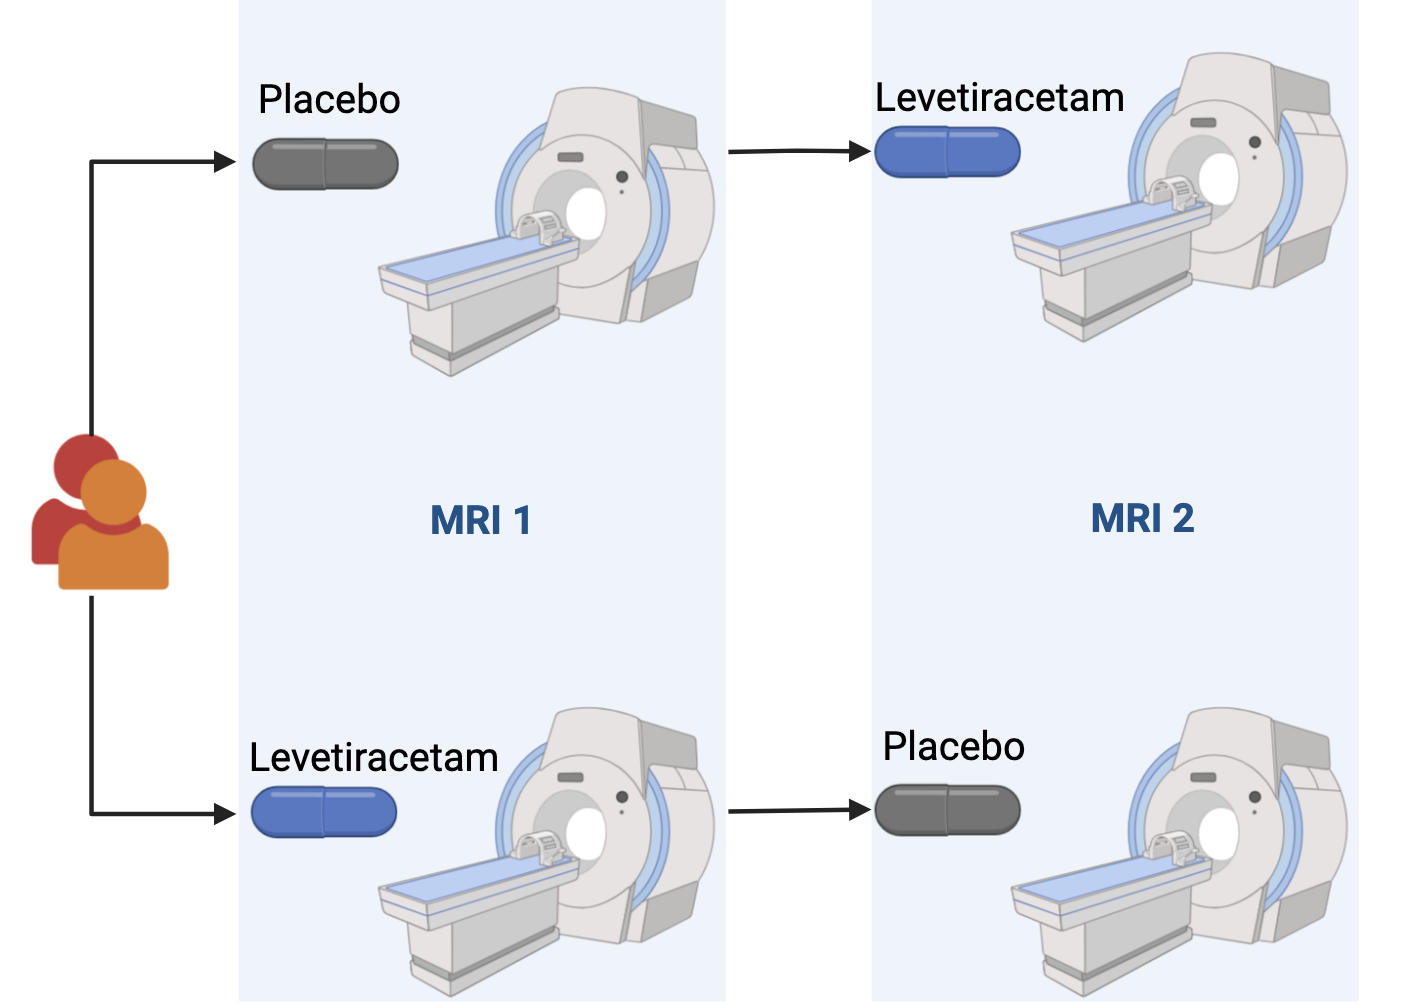
\includegraphics{files/study_design.png}
\end{center}

\subsubsection{Measuring glutamate}\label{measuring-glutamate}

\begin{itemize}
\tightlist
\item
  Glutamate is measured in two voxels localised in the ACC and in the
  Hippocampus. The choice of those regions was based on previous
  findings of decreased SV2A density ({[}11C{]}UCB-J V\(_T\)) in the ACC
  in patients with schizophrenia \autocite{onwordi_synaptic_2020}, and
  an alter relationship between glutamate and SV2A density in the
  hippocampus \autocite{onwordi_relationship_2021}.
\item
  Single voxel spectroscopy (svs) PRESS sequence is used to acquire the
  signal
\item
  I will also report Glx levels to verify if similar differences are
  observed compared to glutamate signal {[}\^{}This is due to limited
  ability to separate glutamine and glutamate using the PRESS sequence
  at 3T{]}.
\end{itemize}

\subsubsection{Behavioural measures}\label{behavioural-measures}

\begin{itemize}
\tightlist
\item
  Change is symptoms is assessed using Positive and Negative Syndrome
  Scale (PANSS).
\item
  PANSS is administered at the screening appointment, and before and
  after every scan, to assess any change in symptoms related to
  levetiracetam.
\end{itemize}

\subsection{Analysis}\label{analysis}

\subsubsection{Change in glutamate}\label{change-in-glutamate}

\begin{itemize}
\tightlist
\item
  MRS data processing will be done in Osprey, and values of Glu (and
  Glx) will be extracted for each participant's scans.
\item
  To compare the changes in levels of glutamate between participants
  with schizophrenia and healthy controls I will do a 2x2 ANOVA.
\item
  I will aso do power calculations. (mention the ones already done).
\item
  I will compare the effect of levetiracetam on Glx levels in healthy
  controls (HC) and patients with schizophrenia (SZ). This will be
  visualised on a raincloud plot such as the one below.
\item
  Below is example of data visualisation. The data used in this graph is
  made up.
\end{itemize}

\begin{figure}

\centering{

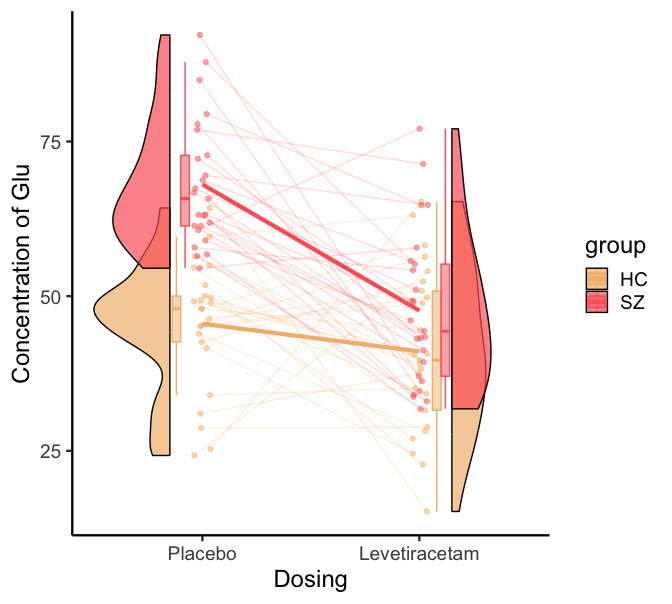
\includegraphics{index_files/figure-latex/notebooks-plots-fig-lev_hc_vs_sz-output-2.png}

}

\caption{\label{fig-lev_hc_vs_sz}Comparison of Glu levels change between
placebo and levetiracetam in HC and SZ}

\end{figure}%

\textsubscript{Source:
\href{https://juliam98.github.io/phd-upgrade-proposal/notebooks/plots-preview.html\#cell-fig-lev_hc_vs_sz}{Plots}}

\subsubsection{Change in symptoms}\label{change-in-symptoms}

\begin{itemize}
\tightlist
\item
  PANSS score for each symptom group and overall PANSS score will be
  calculated for all participants.
\end{itemize}

\section{Progress made to date, including pilot work, if
applicable}\label{progress-made-to-date-including-pilot-work-if-applicable}

\section{Planned future work}\label{planned-future-work}

\section{Contribution to existing
knowledge.}\label{contribution-to-existing-knowledge.}

\textbf{How the research will form a distinct contribution to existing
knowledge on the subject and afford evidence of originality shown by
discovery of new facts or exercise of independent critical power}

\section{Personal share in
investigations}\label{personal-share-in-investigations}

\textbf{Where work is done in conjunction with the supervisor and/or
with collaborators or other students, a statement of the candidate's own
personal share in the investigations}

\section{Timeline for the remainder of
studies.}\label{timeline-for-the-remainder-of-studies.}

\begin{figure}[H]

\centering{

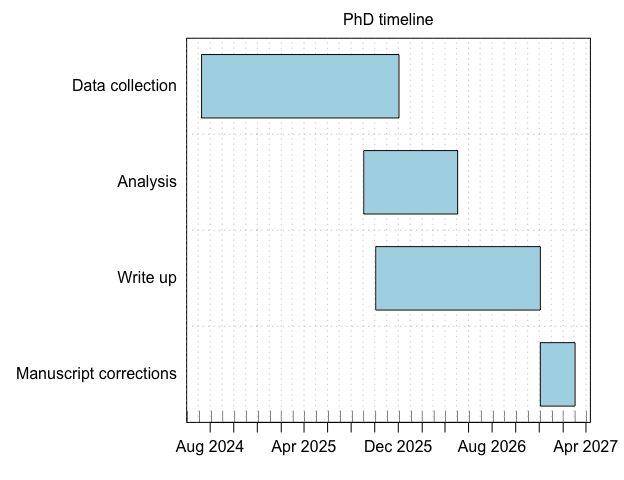
\includegraphics{index_files/figure-latex/notebooks-plots-fig-gantt-chart-output-1.png}

}

\caption{\label{fig-gantt-chart}Gantt chart of planned work during my
PhD}

\end{figure}%

\textsubscript{Source:
\href{https://juliam98.github.io/phd-upgrade-proposal/notebooks/plots-preview.html\#cell-fig-gantt-chart}{Plots}}

\newpage{}

\section{References}\label{references}

\printbibliography[heading=none]




\end{document}
